% ==============================================================================
% ch07.tex -- Chapter 7: Quotients by finite groups
%   Source: book pp. 186--223 (physical pp. 197--234)
% ==============================================================================
\chapter{Quotients by Finite Groups}
\label{ch:7}
\markboth{7.\ \MakeUppercase{Quotients by Finite Groups}}{}

% ------------------------------------------------------------------------------
% Section 7.1
% ------------------------------------------------------------------------------
\section{The general situation}
\label{sec:7.1}

\kmitem\label{item:7.1.1}
Let $R$ be a ring, $G$ a finite group, and $\mathcal{P}$ a moduli problem on \EllR. We say that $G$ \emph{operates} on $\mathcal{P}$ if for every $R$-scheme $S$, and every elliptic curve $E/S$, the group $G$ operates on the set $\mathcal{P}(E/S)$ in such a way that for every morphism in \EllR, viewed as a Cartesian diagram
\[
\begin{tikzcd}[column sep=large, row sep=large]
E_1 \arrow[r, "a"] \arrow[d] & E \arrow[d] \\
S_1 \arrow[r, "f"] & S ,
\end{tikzcd}
\]
the obvious diagram of actions below commutes:
\begin{equation}\label{eq:7.1.1.1}\baretagnumber
\begin{tikzcd}[column sep=huge, row sep=large, every label/.append style={font=\scriptsize}]
G \times \mathcal{P}(E/S) \arrow[r, "\text{action}"] \arrow[d, "{\mathrm{id}\times(a,f)^*}"'] & \mathcal{P}(E/S) \arrow[d, "{(a,f)^*}"] \\
G \times \mathcal{P}(E_1/S_1) \arrow[r, "\text{action}"] & \mathcal{P}(E_1/S_1) .
\end{tikzcd}
\end{equation}
If $\mathcal{P}$ is relatively representable, then for every $E/S$, the group $G$ acts on the $S$-scheme $\mathcal{P}_{E/S}$.

\kmitem\label{item:7.1.2}
Let $\mathcal{P}$ and $\mathcal{P}'$ be two relatively representable moduli problems on which $G$ operates, and let
\[
\mathcal{P} \to \mathcal{P}'
\]
be a $G$-equivariant morphism of moduli problems on \EllR; for every $E/S/R$, we are given a $G$-equivariant map of $G$-sets
\[
\mathcal{P}(E/S) \to \mathcal{P}'(E/S)
\]
compatible with morphisms in \EllR. We say that $\mathcal{P}'$ is ``the'' quotient of $\mathcal{P}$ by $G$, and write $\mathcal{P}' = \mathcal{P}/G$, if the following two conditions hold:
\begin{kmindent}
\noindent\hangindent=3.4em\hangafter=1 (Q1): $G$ operates trivially on $\mathcal{P}'$.

\noindent\hangindent=3.4em\hangafter=1 (Q2): For every representable moduli problem $\mathcal{S}$ on \EllR\ which is etale over \EllR, the quotient scheme $\Mfrak(\mathcal{S},\mathcal{P})/G$ exists, and it maps isomorphically to $\Mfrak(\mathcal{S},\mathcal{P}')$. [Equivalently: for every modular family of elliptic curves $\mathcal{E}/\mathcal{S}/R$, the quotient scheme $(\mathcal{P}_{\mathcal{E}/\mathcal{S}})/G$ exists, and maps isomorphically to $(\mathcal{P}')_{\mathcal{E}/\mathcal{S}}$.]
\end{kmindent}

\begin{kthm}\label{thm:7.1.3}
Let $\mathcal{P}$ be relatively representable and affine over \EllR, and $G$ a finite group acting on $\mathcal{P}$. Then
\begin{enumerate}[(1)]
\item The quotient $\mathcal{P}/G$ exists as a relatively representable moduli problem, affine over \EllR. For any relatively representable $\mathcal{P}'$, with trivial $G$-action, any $G$-equivariant map $\mathcal{P} \to \mathcal{P}'$ factors uniquely through the projection $\mathcal{P} \to \mathcal{P}/G$, so that $\mathcal{P}/G$ represents the covariant functor on the category of all relatively representable moduli problems with trivial $G$-action defined by
\[
\mathcal{P}' \mapsto \Hom_{G\text{-equiv}}(\mathcal{P}, \mathcal{P}') .
\]
\item If $G$ operates freely on $\mathcal{P}$, in the sense that for every $E/S/R$, $G$ operates freely on the set $\mathcal{P}(E/S)$, then $\mathcal{P}$ is an etale $G$-torsor over $\mathcal{P}/G$; for every $E/S/R$, $G$ operates freely on the $S$-scheme $\mathcal{P}_{E/S}$, $\mathcal{P}_{E/S}$ is an etale $G$-torsor over $(\mathcal{P}/G)_{E/S}$, and $(\mathcal{P}_{E/S})/G \xrightarrow{\ \sim\ } (\mathcal{P}/G)_{E/S}$.
\item For any $E/S/R$, the quotient scheme $\mathcal{P}_{E/S}/G$ exists, and there is a natural $S$-morphism
\[
(\mathcal{P}_{E/S})/G \to (\mathcal{P}/G)_{E/S} ,
\]
which is bijective on geometric points. It is an isomorphism if any of the following conditions hold:
\begin{enumerate}[a)]
\item $E/S$ is (as representable moduli problem) flat over \EllR;
\item the order of $G$ is invertible on $S$;
\item $G$ operates freely on $\mathcal{P}$.
\end{enumerate}
\item The morphism $\mathcal{P} \to \mathcal{P}/G$ is finite.
\item If $\mathcal{P}$ is normal, so is $\mathcal{P}/G$.
\item If $\mathcal{P}$ is finite over \EllR, and $R$ is noetherian, then $\mathcal{P}/G$ is finite over \EllR.
\end{enumerate}
\end{kthm}

\begin{proof}[Construction-proof]
Let us denote by $(\Sch/R\text{-}\Sch)$ the category whose objects are $R$-morphisms of $R$-schemes
\[
\kmobj{X}{S} \qquad S \text{ an } R\text{-scheme}
\]
and whose morphisms are cartesian squares of $R$-schemes
\[
\begin{tikzcd}[column sep=large, row sep=large]
X_1 \arrow[r, "a"] \arrow[d] & X \arrow[d] \\
S_1 \arrow[r, "f"] & S .
\end{tikzcd}
\]
We denote by
\[
\mathrm{Base} : (\Sch/R\text{-}\Sch) \to (R\text{-}\Sch)
\]
the functor
\[
\kmobj{E}{S}
\]
When no confusion is possible, we also denote by
\[
\mathrm{Base} : \EllR \to (R\text{-}\Sch) ,
\]
the analogous functor
\[
\kmobj{\mathcal{P}_{E/S}}{S}
\]
A covariant functor
\[
\mathcal{F} : \EllR \to (\Sch/R\text{-}\Sch)
\]
is called \emph{base-preserving} if the diagram
\[
\begin{tikzcd}[column sep=huge, row sep=large]
\EllR \arrow[r, "\mathcal{F}"] \arrow[rd, "\mathrm{Base}"'] & (\Sch/R\text{-}\Sch) \arrow[d, "\mathrm{Base}"] \\
& (R\text{-}\Sch)
\end{tikzcd}
\]
is commutative.

Given a relatively representable moduli problem $\mathcal{P}$ on \EllR, we denote by $\mathcal{P}^{\Sch}$ the base-preserving functor
\[
\mathcal{P}^{\Sch} : \EllR \to (\Sch/R\text{-}\Sch)
\]
defined by
\[
\kmfobj{E}{\mathcal{P}_{E/S}}{S}
\]
The construction
\[
\mathcal{P} \mapsto \mathcal{P}^{\Sch}
\]
defines an equivalence of categories
\[
\left(\begin{array}{@{}c@{}}
\text{relatively repre-} \\[-1pt]
\text{sentable problems} \\[-1pt]
\text{on \EllR}
\end{array}\right) \xrightarrow{\ \sim\ }
\left(\begin{array}{@{}c@{}}
\text{base-preserving} \\[-1pt]
\text{functors from} \\[-1pt]
\text{\EllR\ to $(\Sch/R\text{-}\Sch)$}
\end{array}\right) .
\]
The inverse construction associates to a base-preserving functor $\mathcal{F}$ the relatively representable moduli problem $\mathcal{P}$ defined by
\[
\mathcal{P}(E/S) = \Hom_{S\text{-}\Sch}(S, \mathcal{F}_{E/S}) ,
\]
so that
\[
\mathcal{P}_{E/S} = \mathcal{F}_{E/S} .
\]

We will make use of this equivalence to discuss the case of a finite group $G$ acting freely on a relatively representable moduli problem $\mathcal{P}$ which is affine over \EllR. In this case, $G$ operates freely and $S$-linearly on the affine $S$-scheme $\mathcal{P}_{E/S}$, for every $E/S/R$. By \cite[III, \S2,6.1]{DeGa}, we know that if a finite group $G$ operates freely and $S$-linearly on an affine $S$-scheme $X$, then the quotient $X/G$ exists, $X$ is a finite etale $G$-torsor over $X/G$, and the formation of $X/G$ commutes with arbitrary base-change $S' \to S$. Therefore the construction
\[
\kmfobj{E}{(\mathcal{P}_{E/S})/G}{S}
\]
defines a base-preserving functor
\[
\mathcal{P}^{\Sch}/G : \EllR \to (\Sch/R\text{-}\Sch) ,
\]
whose associated relatively representable moduli problem we define to be $\mathcal{P}/G$, so that
\[
(\mathcal{P}/G)^{\Sch} = \mathcal{P}^{\Sch}/G .
\]
It is clear that this $\mathcal{P}/G$ does indeed have the universal property required in (1) of the theorem, and that (2) of the theorem holds.

We now consider the general case, when $G$ is no longer assumed to act freely on $\mathcal{P}$. The problem of constructing $\mathcal{P}/G$ satisfying (1) is clearly Zariski local on $R$, so we may assume that an odd prime $\ell$ is invertible in $R$. Consider the simultaneous problem $([\Gamma(\ell)], \mathcal{P})$. It is representable because it maps to the representable problem $[\Gamma(\ell)]$, the product group $\GL(2,\F_\ell) \times G$ operates on it, and the first factor $\GL(2,\F_\ell)$ operates freely on it (because $\GL(2,\F_\ell)$ operates freely on $[\Gamma(\ell)]$ over any ring $R$ in which $\ell$ invertible, cf.\ (\ref{cor:3.7.2})).

By the above discussion of the quotient by a free action, we may recover $\mathcal{P}$ from the simultaneous problem $([\Gamma(\ell)], \mathcal{P})$ with its action of $\GL(2,\F_\ell)$ by the rule
\[
([\Gamma(\ell)], \mathcal{P})/\GL(2,\F_\ell) \times 1 \xrightarrow{\ \sim\ } \mathcal{P} .
\]
Therefore the construction
\[
\mathcal{P} \mapsto ([\Gamma(\ell)], \mathcal{P}) \quad \text{with action of } \GL(2,\F_\ell)
\]
defines an equivalence of categories
\[
\left(\begin{array}{@{}c@{}}
\text{relatively representable} \\[-1pt]
\text{moduli problems $\mathcal{P}$ on} \\[-1pt]
\text{\EllR}
\end{array}\right) \xrightarrow{\ \sim\ }
\left(\begin{array}{@{}c@{}}
\text{representable moduli} \\[-1pt]
\text{problems $\mathcal{S}$ on \EllR} \\[-1pt]
\text{given with an action of} \\[-1pt]
\text{$\GL(2,\F_\ell)$ and with a} \\[-1pt]
\text{$\GL(2,\F_\ell)$-equivariant map} \\[-1pt]
\text{to $[\Gamma(\ell)] \otimes R$.}
\end{array}\right)
\]
Passing to modular schemes defines an equivalence
\[
\left(\begin{array}{@{}c@{}}
\text{representable moduli} \\[-1pt]
\text{problems $\mathcal{S}$ on \EllR} \\[-1pt]
\text{given with an action of} \\[-1pt]
\text{$\GL(2,\F_\ell)$ and with a} \\[-1pt]
\text{$\GL(2,\F_\ell)$-equivariant map} \\[-1pt]
\text{to $[\Gamma(\ell)] \otimes R$.}
\end{array}\right) \xrightarrow{\ \sim\ }
\left(\begin{array}{@{}c@{}}
\text{$\Mfrak(\Gamma(\ell)) \otimes R$-schemes} \\[-1pt]
\text{given with an action} \\[-1pt]
\text{of $\GL(2,\F_\ell)$ covering} \\[-1pt]
\text{its standard action on} \\[-1pt]
\text{$\Mfrak(\Gamma(\ell)) \otimes R$.}
\end{array}\right) ,
\]
\[
\mathcal{S} \mapsto \Mfrak(\mathcal{S}) .
\]
By means of this last equivalence an action of a finite group $G$ on a relatively representable $\mathcal{P}$ which is affine over \EllR\ corresponds to an $\Mfrak(\Gamma(\ell)) \otimes R$-linear action of $G$ on an affine $\Mfrak(\Gamma(\ell)) \otimes R$-scheme $\Mfrak(\mathcal{S})$ which commutes with the given action of $\GL(2,\F_\ell)$ on $\Mfrak(\mathcal{S})$. Viewed in this way, it is clear that the quotient of $\mathcal{P}$ by $G$ exists and satisfies the required universal property; it corresponds under this equivalence to the quotient $\Mfrak(\mathcal{S})/G$ with its induced action of $\GL(2,\F_\ell)$ and its $\GL(2,\F_\ell)$-equivariant map to $\Mfrak(\Gamma(\ell)) \otimes R$:
\[
\begin{tikzcd}[column sep=large, row sep=large]
\Mfrak(\mathcal{S}) \arrow[d] \\
\Mfrak(\mathcal{S})/G \arrow[d] \\
\Mfrak(\Gamma(\ell)) \otimes R .
\end{tikzcd}
\]
This concludes the proof of parts (1) and (2) of the theorem.

``Concretely'', for any representable problem $\mathcal{S}$ on \EllR, the $\Mfrak(\mathcal{S})$-scheme $\Mfrak(\mathcal{S}, \mathcal{P}/G)$ is constructed in three steps:
\begin{kmindent}
\noindent\hangindent=3.2em\hangafter=1 (a) $\Mfrak(\mathcal{S}, \mathcal{P}/G) = \Mfrak(\mathcal{S}, \Gamma(\ell), \mathcal{P}/G)/\GL(2,\F_\ell)$

\noindent\hangindent=3.2em\hangafter=1 (b) $\Mfrak(\mathcal{S}, \Gamma(\ell), \mathcal{P}/G) = \Mfrak(\mathcal{S}, \Gamma(\ell)) \underset{\Mfrak(\Gamma(\ell))}{\times} \Mfrak(\Gamma(\ell), \mathcal{P}/G)$

\noindent\hangindent=3.2em\hangafter=1 (c) $\Mfrak(\Gamma(\ell), \mathcal{P}/G) = \Mfrak(\Gamma(\ell), \mathcal{P})/G$.
\end{kmindent}
Thus all in all we have
\[
\Mfrak(\mathcal{S}, \mathcal{P}/G) = \left( \Mfrak(\mathcal{S}, \Gamma(\ell)) \underset{\Mfrak(\Gamma(\ell))}{\times} \left( \Mfrak(\Gamma(\ell), \mathcal{P})/G \right) \right) \Big/ \GL(2,\F_\ell) ,
\]
while computing $\Mfrak(\mathcal{S}, \mathcal{P})$ this way leads to
\[
\Mfrak(\mathcal{S}, \mathcal{P}) = \left( \Mfrak(\mathcal{S}, \Gamma(\ell)) \underset{\Mfrak(\Gamma(\ell))}{\times} \Mfrak(\Gamma(\ell), \mathcal{P}) \right) \Big/ \GL(2,\F_\ell) ,
\]
and so
\[
\begin{aligned}
\Mfrak(\mathcal{S}, \mathcal{P})/G
  &= \bigl( \Mfrak(\mathcal{S}, \Gamma(\ell)) \underset{\Mfrak(\Gamma(\ell))}{\times} \Mfrak(\Gamma(\ell), \mathcal{P}) \bigr) \big/ \GL(2,\F_\ell) \times G \\
  &= \Bigl( \bigl( \Mfrak(\mathcal{S}, \Gamma(\ell)) \underset{\Mfrak(\Gamma(\ell))}{\times} \Mfrak(\Gamma(\ell), \mathcal{P}) \bigr) \big/ G \Bigr) \big/ \GL(2,\F_\ell) .
\end{aligned}
\]
The canonical morphism from $\Mfrak(\mathcal{S}, \mathcal{P})/G$ to $\Mfrak(\mathcal{S}, \mathcal{P}/G)$ is just the one deduced from passage to $\GL(2,\F_\ell)$-invariant from the morphism
\[
\begin{aligned}
&\bigl( \Mfrak(\mathcal{S}, \Gamma(\ell)) \underset{\Mfrak(\Gamma(\ell))}{\times} \Mfrak(\Gamma(\ell), \mathcal{P}) \bigr) \Big/ G \\
&\qquad \to \Mfrak(\mathcal{S}, \Gamma(\ell)) \underset{\Mfrak(\Gamma(\ell))}{\times} \bigl( \Mfrak(\Gamma(\ell), \mathcal{P})/G \bigr) .
\end{aligned}
\]
The question of when this morphism is an isomorphism, or a bijection on geometric points, is the question of the extent to which formation of rings of invariants commutes with extension of scalars.

The results of (3) follow immediately from the standard facts about this question, which are given in (\ref{sec:A.7}). In the same vein, (4), (5), and (6) are simply translations of the following facts:
\begin{kmindent}
\noindent\hangindent=4.6em\hangafter=1 for (4): take any modular $E/S$ with $S$ affine, $S = \Spec(B)$; then $\mathcal{P}_{E/S}$ is $\Spec(A)$ for some $B$-algebra $A$ of finite presentation, upon which $G$ acts $B$-linearly. Therefore $A$ is finitely generated as an $A^G$-algebra. Visibly every element $a$ of $A$ is integral over $A^G$, being a root of the $A^G$-polynomial
\[
\prod_{g} (\mathrm{T} - g(a)) .
\]
Therefore $A$ is finite as an $A^G$-module.

\noindent\hangindent=4.6em\hangafter=1 for (5): This says $A^G$ is normal if $A$ is.

\noindent\hangindent=4.6em\hangafter=1 for (6): If $A$ is a finite $B$-module, and if $B$ is noetherian, then $A^G \subset A$ is a sub-$B$-module, so also finite over $B$. Q.E.D.
\end{kmindent}
\end{proof}

\begin{krem}\label{rem:7.1.4}
If $R \to R'$ is a ring homomorphism, then for $\mathcal{P}$ and $G$ as in the theorem there is a natural morphism
\[
(\mathcal{P} \underset{R}{\otimes} R')/G \to (\mathcal{P}/G) \underset{R}{\otimes} R'
\]
of moduli problems on $(\mathrm{Ell}/R')$, which is an isomorphism if $R \to R'$ is flat, or if the order of $G$ is invertible in $R'$, or if $G$ acts freely on $\mathcal{P}$. It is always surjective and radicial.
\end{krem}

\begin{kcor}\label{cor:7.1.5}
Suppose that $R$ is noetherian. Let $\mathfrak{p}$ be a prime ideal of $R$, $k_0$ its residue field, $k$ a separable closure of $k_0$, and $\widehat{R}$ the completion of the strict henselization of the local ring at $\mathfrak{p}$. For any elliptic curve $E/k$, let $E/\widehat{R}[[T]]$ be its universal formal deformation (to artin local $\widehat{R}$-algebras with residue field $k$). If $\mathcal{P}$ is relatively representable and affine over $(\mathrm{Ell}/R)$, and if $G$ is a finite group acting on $\mathcal{P}$, then we have a canonical isomorphism of $\widehat{R}[[T]]$-schemes
\[
(\mathcal{P}_{E/\widehat{R}[[T]]})/G \xrightarrow{\ \sim\ } (\mathcal{P}/G)_{E/\widehat{R}[[T]]} .
\]
\end{kcor}

\begin{proof}
Choose an odd prime $\ell \neq \mathrm{char}(k)$, which we may assume invertible on $R$. Then the moduli problem $\mathcal{S} = [\Gamma(\ell)] \underset{\Z}{\otimes} R$ is finite etale over $(\mathrm{Ell}/R)$. Fix a $\Gamma(\ell)$-structure on $E/k$. It extends uniquely to a $\Gamma(\ell)$-structure on $E/\widehat{R}[[T]]$, and with it we may view $\widehat{R}[[T]]$ as the completion of the strict henselization of $\Mfrak(\mathcal{S})$ at the image of the point $(E/k$, its $\Gamma(\ell)$-structure$)$. Consider the diagram of schemes over $\Mfrak(\mathcal{S})$
\[
\begin{tikzcd}[column sep=huge, row sep=large]
\Mfrak(\mathcal{S}, \mathcal{P}) \arrow[r] \arrow[rd] & \Mfrak(\mathcal{S}, \mathcal{P}/G) = \Mfrak(\mathcal{S}, \mathcal{P})/G \arrow[d] \\
& \Mfrak(\mathcal{S}) ,
\end{tikzcd}
\]
Because $\widehat{R}[[T]]$ is flat over $\Mfrak(\mathcal{S})$, we have
\[
\left( \Mfrak(\mathcal{S}, \mathcal{P}) \underset{\Mfrak(\mathcal{S})}{\times} \widehat{R}[[T]] \right) \Big/ G \xrightarrow{\ \sim\ } \left( \Mfrak(\mathcal{S}, \mathcal{P})/G \right) \underset{\Mfrak(\mathcal{S})}{\times} \widehat{R}[[T]] ,
\]
which is none other than the desired isomorphism
\[
(\mathcal{P}_{E/\widehat{R}[[T]]})/G \xrightarrow{\ \sim\ } (\mathcal{P}/G)_{E/\widehat{R}[[T]]} .
\]
\end{proof}

% ------------------------------------------------------------------------------
% Section 7.2
% ------------------------------------------------------------------------------
\section{A descent situation}
\label{sec:7.2}

\kmitem\label{item:7.2.1}
Let $\mathcal{P}$ and $\mathcal{P}'$ be relatively representable and affine over \EllR. Suppose that a finite group $G$ acts on both $\mathcal{P}$ and $\mathcal{P}'$, and that we are given a $G$-equivariant morphism
\[
\mathcal{P} \to \mathcal{P}' .
\]

\begin{kprop}\label{prop:7.2.2}
If $G$ operates freely on $\mathcal{P}'$, then the natural map
\[
\mathcal{P}/G \to \mathcal{P}'/G
\]
sits in a cartesian diagram
\[
\begin{tikzcd}[column sep=huge, row sep=large]
\mathcal{P} \arrow[r] \arrow[d] & \mathcal{P}/G \arrow[d] \\
\mathcal{P}' \arrow[r] & \mathcal{P}'/G ,
\end{tikzcd}
\]
i.e., for every $E/S$ the diagram of $S$-schemes
\[
\begin{tikzcd}[column sep=huge, row sep=large]
\mathcal{P}_{E/S} \arrow[r] \arrow[d] & (\mathcal{P}/G)_{E/S} \arrow[d] \\
\mathcal{P}'_{E/S} \arrow[r] & (\mathcal{P}'/G)_{E/S}
\end{tikzcd}
\]
is cartesian.
\end{kprop}

\begin{proof}
Because $G$ operates freely on $\mathcal{P}'$, we know that for every $E/S$, $\mathcal{P}'_{E/S}$ is an etale $G$-torsor over $(\mathcal{P}'/G)_{E/S} = (\mathcal{P}'_{E/S})/G$. By etale descent, it is the same to give a $(\mathcal{P}'/G)_{E/S}$-scheme $Z_2$ as it is to give a $\mathcal{P}'_{E/S}$-scheme $Z_1$ together with a lifting of the action of $G$, the two related by
\[
Z_2 = Z_1/G, \quad Z_1 = \left( Z_2 \underset{(\mathcal{P}'/G)_{E/S}}{\times} (\mathcal{P}')_{E/S} \right) .
\]
Take for $Z_1$ the scheme $\mathcal{P}_{E/S}$. The associated $Z_2$ which fits into the cartesian diagram is $Z_1/G = (\mathcal{P}_{E/S})/G$. But because $G$ acts freely on $\mathcal{P}'$ it acts all the more freely on $\mathcal{P}$, so we do indeed have $Z_2 = (\mathcal{P}/G)_{E/S}$ by (\ref{thm:7.1.3}, 3(c)).
\end{proof}

% ------------------------------------------------------------------------------
% Section 7.3
% ------------------------------------------------------------------------------
\section{Quotients of product problems}
\label{sec:7.3}

\begin{kprop}\label{prop:7.3.1}
Let $\mathcal{P}_1$ and $\mathcal{P}_2$ be two relatively representable moduli problems affine over \EllR. Suppose that finite groups $G_1$ and $G_2$ operate on $\mathcal{P}_1$ and $\mathcal{P}_2$ respectively, that $\mathcal{P}_1$ is flat over \EllR, and that $\mathcal{P}_2/G_2$ is flat over \EllR.

Then we have a canonical isomorphism
\[
(\mathcal{P}_1, \mathcal{P}_2)/(G_1 \times G_2) \xrightarrow{\ \sim\ } (\mathcal{P}_1/G_1, \mathcal{P}_2/G_2) .
\]
\end{kprop}

\begin{proof}
Let $\mathcal{S}$ be a representable problem, etale over \EllR. By definition of quotients we have
\[
\begin{aligned}
\Mfrak(\mathcal{S}, (\mathcal{P}_1, \mathcal{P}_2)/G_1 \times G_2) &= \Mfrak(\mathcal{S}, \mathcal{P}_1, \mathcal{P}_2)/G_1 \times G_2 \\
&= \bigl( \Mfrak(\mathcal{S}, \mathcal{P}_1) \underset{\Mfrak(\mathcal{S})}{\times} \Mfrak(\mathcal{S}, \mathcal{P}_2) \bigr) \big/ G_1 \times G_2 ,
\end{aligned}
\]
while
\[
\begin{aligned}
\Mfrak(\mathcal{S}, \mathcal{P}_1/G_1, \mathcal{P}_2/G_2)
  &= \Mfrak(\mathcal{S}, \mathcal{P}_1/G_1) \underset{\Mfrak(\mathcal{S})}{\times} \Mfrak(\mathcal{S}, \mathcal{P}_2/G_2) \\
  &= \left( \Mfrak(\mathcal{S}, \mathcal{P}_1)/G_1 \right) \underset{\Mfrak(\mathcal{S})}{\times} \left( \Mfrak(\mathcal{S}, \mathcal{P}_2)/G_2 \right) .
\end{aligned}
\]
If $\Spec(B)$ is an affine open of $\Mfrak(\mathcal{S})$, and if $\Spec(A_1)$ and $\Spec(A_2)$ are its inverse images in $\Mfrak(\mathcal{S}, \mathcal{P}_1)$ and $\Mfrak(\mathcal{S}, \mathcal{P}_2)$ respectively, then the natural map $(\mathcal{P}_1, \mathcal{P}_2)/G_1 \times G_2 \to (\mathcal{P}_1/G_1, \mathcal{P}_2/G_2)$ is given on affine rings by
\[
(A_1)^{G_1} \otimes_B (A_2)^{G_2} \to (A_1 \otimes_B A_2)^{G_1 \times G_2} .
\]
By hypothesis, $A_1$ and $(A_2)^{G_2}$ are both flat over $B$. Therefore
\[
\begin{aligned}
(A_1 \otimes_B A_2)^{G_1 \times G_2}
  &= \left( (A_1 \otimes_B A_2)^{G_2} \right)^{G_1} \\
  &= \left( A_1 \otimes_B (A_2)^{G_2} \right)^{G_1} \\
  &= (A_1)^{G_1} \otimes_B (A_2)^{G_2} .
\end{aligned}
\]
\end{proof}

% ------------------------------------------------------------------------------
% Section 7.4
% ------------------------------------------------------------------------------
\section{Applications to the four basic moduli problems}
\label{sec:7.4}

\kmitem\label{item:7.4.1}
Let $N \ge 1$ be an integer. The group $\GL(2,\Z/N\Z)$ operates on the moduli problem $[\Gamma(N)]$, through its right action on Drinfeld bases: $\gamma = \begin{pmatrix} a & b \\ c & d \end{pmatrix} \in \GL(2,\Z/N\Z)$ acts by
\[
(P, Q) \mapsto (P, Q) \begin{pmatrix} a & b \\ c & d \end{pmatrix} = (aP + cQ, bP + dQ) .
\]
This action is well defined, for it leaves unchanged the Cartier divisor
\[
\sum_{\substack{n, m \bmod N}} [nP + mQ] .
\]
The group $(\Z/N\Z)^\times \times (\Z/N\Z)^\times$ operates on the moduli problem $[\mathrm{bal.}\ \Gamma_1(N)]$, through its action on the generators: an element $(a,b)$ of this group acts as
\[
\left( P\ ;\ E \xrightarrow[\pi^t]{\pi} E'\ ;\ P' \right) \mapsto \left( aP\ ;\ E \xrightarrow[\pi^t]{\pi} E'\ ;\ bP' \right) .
\]
The group $(\Z/N\Z)^\times$ operates on the moduli problem $[\Gamma_1(N)]$ through its action on the given generator; an element $a$ acts as
\[
(E, P) \mapsto (E, aP) .
\]

\begin{kthm}\label{thm:7.4.2}
Let $N \ge 1$ be an integer. Then
\begin{enumerate}[(1)]
\item For any divisor $d$ of $N$, the natural map
\[
\begin{aligned}
& [\Gamma(N)] \to [\Gamma(d)] \\
& \quad (P, Q) \mapsto ((N/d)P, (N/d)Q)
\end{aligned}
\]
identifies $[\Gamma(d)]$ with the quotient of $[\Gamma(N)]$ by the principal congruence subgroup of $\GL(2,\Z/N\Z)$ consisting of those elements $\equiv \mathrm{id} \bmod d$.
\item The natural map
\[
\begin{aligned}
& [\Gamma(N)] \to [\mathrm{bal.}\ \Gamma_1(N)] \\
& \quad (P, Q) \mapsto (P, Q \bmod P)
\end{aligned}
\]
identifies $[\mathrm{bal.}\ \Gamma_1(N)]$ with the quotient of $[\Gamma(N)]$ by the unipotent subgroup $\begin{pmatrix} 1 & * \\ 0 & 1 \end{pmatrix}$ of $\GL(2,\Z/N\Z)$.
\item The natural map
\[
\begin{aligned}
& [\Gamma(N)] \to [\Gamma_1(N)] \\
& \quad (P, Q) \mapsto P
\end{aligned}
\]
identifies $[\Gamma_1(N)]$ with the quotient of $[\Gamma(N)]$ by the ``semi-Borel'' subgroup $\begin{pmatrix} 1 & * \\ 0 & * \end{pmatrix}$ of $\GL(2,\Z/N\Z)$.
\item The natural map
\[
\begin{aligned}
& [\Gamma(N)] \to [\Gamma_0(N)] \\
& \quad (P, Q) \mapsto \text{subgroup ``generated'' by } P
\end{aligned}
\]
identifies $[\Gamma_0(N)]$ with the quotient of $[\Gamma(N)]$ by the Borel subgroup $\begin{pmatrix} * & * \\ 0 & * \end{pmatrix}$ of $\GL(2,\Z/N\Z)$.
\item The natural map
\[
\begin{aligned}
& [\mathrm{bal.}\ \Gamma_1(N)] \to [\Gamma_1(N)] \\
& \quad \left( P\ ;\ E \xrightarrow[\pi^t]{\pi} E'\ ;\ P' \right) \longmapsto (E, P)
\end{aligned}
\]
identifies $[\Gamma_1(N)]$ as the quotient of $[\mathrm{bal.}\ \Gamma_1(N)]$ by the subgroup $1 \times (\Z/N\Z)^\times$ of $(\Z/N\Z)^\times \times (\Z/N\Z)^\times$.
\item The natural map
\[
\begin{aligned}
& [\mathrm{bal.}\ \Gamma_1(N)] \to [\Gamma_0(N)] \\
& \quad \left( P\ ;\ E \xleftarrow[\pi^t]{} E'\ ;\ P' \right) \longmapsto (E, \Ker(\pi))
\end{aligned}
\]
identifies $[\Gamma_0(N)]$ with the quotient of $[\mathrm{bal.}\ \Gamma_1(N)]$ by $(\Z/N\Z)^\times \times (\Z/N\Z)^\times$.
\item The natural map
\[
\begin{aligned}
& [\Gamma_1(N)] \to [\Gamma_0(N)] \\
& \quad (E, P) \mapsto (E, \text{subgroup generated by } P)
\end{aligned}
\]
identifies $[\Gamma_0(N)]$ with the quotient of $[\Gamma_1(N)]$ by $(\Z/N\Z)^\times$.
\end{enumerate}
\end{kthm}

\begin{proof}
We will prove (1). The other proofs are entirely analogous, and are left to the reader. Let $G$ denote the mod $d$ congruence subgroup of $\GL(2,\Z/N\Z)$. The given morphism
\[
[\Gamma(N)] \to [\Gamma(d)]
\]
is $G$-equivariant, with $G$ acting trivially on $[\Gamma(d)]$. We must show that for any representable moduli problem $\mathcal{S}$ which is etale over \Ell, the induced map of $\Mfrak(\mathcal{S})$-schemes
\[
\Mfrak(\mathcal{S}, \Gamma(N))/G \to \Mfrak(\mathcal{S}, \Gamma(d))
\]
is an isomorphism. This is obviously the case if $N$ is invertible, and both sides are normal schemes finite over $\Mfrak(\mathcal{S})$. Therefore they and the map between them are obtained from the isomorphism of finite etale $\Mfrak(\mathcal{S}) \otimes \Z[1/N]$-schemes
{\footnotesize
\[
\begin{tikzcd}[column sep=small, row sep=large, every label/.append style={font=\scriptsize}]
\left( \Mfrak(\mathcal{S}, \Gamma(N)) \otimes \Z[1/N] \right)/G \arrow[rr, "\sim"] \arrow[rd] & & \Mfrak(\mathcal{S}, \Gamma(d)) \otimes \Z[1/N] \arrow[ld] \\
& \Mfrak(\mathcal{S}) \otimes \Z[1/N] &
\end{tikzcd}
\]}
by normalizing $\Mfrak(\mathcal{S})$.
\end{proof}

\kmitem\label{item:7.4.3}
\emph{Summarizing diagram}
\begin{center}
\begin{tikzpicture}[x=1cm, y=1cm, every node/.style={inner sep=1pt, font=\small}]
\node (A) at (3.5, 7.7) {$[\Gamma(N)]$};
\node (B) at (3.5, 6.0) {$[\mathrm{bal.}\ \Gamma_1(N)]$};
\node (C) at (3.5, 4.3) {$[\Gamma_1(N)]$};
\node (D) at (3.5, 2.6) {$[\Gamma_0(N)]$};
\node (E) at (3.5, 0.7) {$[\Gamma_0(1)] = \Ell$};
\node (F) at (8.6, 3.0) {$[\Gamma(d)]$};
\draw[->] (A) to[bend right=30] (B);
\draw[->] (A) to[bend right=40] (C);
\draw[->] (A) to[bend right=50] (D);
\draw[->] (A) to[bend left=32] (F);
\draw[->] (B) to[bend right=26] (C);
\draw[->] (B) to[bend right=40] (D);
\draw[->] (C) to[bend right=26] (D);
\draw[->] (D) -- (E);
\draw[->] (F) to[bend right=20] (E);
\draw[->] (F) to[bend right=30] (E);
\node at (2.45, 6.85) {$\bigl(\begin{smallmatrix}1 & * \\ 0 & 1\end{smallmatrix}\bigr)$};
\node at (1.55, 5.15) {$\bigl(\begin{smallmatrix}1 & * \\ 0 & *\end{smallmatrix}\bigr)$};
\node at (0.65, 3.45) {$\bigl(\begin{smallmatrix}* & * \\ 0 & *\end{smallmatrix}\bigr)$};
\node[anchor=west] at (4.6, 5.15) {$1 \times (\Z/N\Z)^\times$};
\node[anchor=west] at (4.6, 3.45) {$(\Z/N\Z)^\times$};
\node[anchor=west] at (6.1, 4.3) {$(\Z/N\Z)^\times \times (\Z/N\Z)^\times$};
\node[anchor=west] at (6.7, 6.3) {$\GL(2,\Z/N\Z)$};
\end{tikzpicture}
\end{center}

% ------------------------------------------------------------------------------
% Section 7.5
% ------------------------------------------------------------------------------
\section{Axiomatics}
\label{sec:7.5}

\begin{arqt}\label{thm:7.5.1}
Let $\mathcal{P}$ be a relatively representable moduli problem on \Ell, which satisfies axioms Reg.~1, Reg.~2, Reg.~3, Reg.~4A, Reg.~4B of \ref{thm:5.1.1} with respect to some prime $p$. Let $G$ be a finite group which operates on $\mathcal{P}$. Suppose that this $G$-action satisfies the following three axioms:
\begin{kmindent}
\noindent\hangindent=3.6em\hangafter=1 (G-1)\quad $G$ acts freely on $\mathcal{P} \tens{\Z} \Z[1/p]$.

\noindent\hangindent=3.6em\hangafter=1 (G-2)\quad The action of $G$ on $\mathcal{P}$ depends only upon the underlying $p$-divisible group, in the sense that for any two elliptic curves over a common base, say $E/S$ and $E'/S$, and any $S$-isomorphism of their $p$-divisible groups
\[
E[p^\infty] \xrightarrow{\ \sim\ } E'[p^\infty] ,
\]
there exists an isomorphism (cf.\ Reg.~3) of $S$-schemes
\[
\mathcal{P}_{E'/S} \xrightarrow{\ \sim\ } \mathcal{P}_{E/S}
\]
which is $G$-equivariant.

\noindent\hangindent=3.6em\hangafter=1 (G-3)\quad Let $k$ be any algebraically closed field of characteristic $p$, $E_0/k$ any supersingular elliptic curve, $E/W[[T]]$ its universal formal deformation, and $A$ the complete local (Reg.~4A) ring such that $\mathcal{P}_{E/W[[T]]} = \Spec(A)$. Then $A$ is a finite module over $A^G$, generated by $\#G$ elements.
\end{kmindent}
\noindent Then
\begin{enumerate}[(1)]
\item The quotient $\mathcal{P}/G$ is finite and flat over \Ell\ of constant rank $\geq 1$, and regular (necessarily of dimension two).
\item The morphism of moduli problems over \Ell
\[
\mathcal{P} \to \mathcal{P}/G
\]
is finite and flat of degree $\#G$. Outside of $p$, this morphism makes $\mathcal{P}$ into an etale $G$-torsor.
\item The ``complete local ring of $\mathcal{P}/G$ at a supersingular $E_0/k$'' is given by $A^G$, i.e., we have $\Spec(A^G) = (\mathcal{P}/G)_{E/W[[T]]}$ for $E/W[[T]]$ as in axiom G-3.
\item For any elliptic curve $E/k$ with $k$ the algebraic closure of a finite field, and universal formal deformation $E/W[[T]]$, we have an isomorphism of $W[[T]]$-schemes
\[
(\mathcal{P}_{E/W[[T]]})/G \xrightarrow{\ \sim\ } (\mathcal{P}/G)_{E/W[[T]]} .
\]
\end{enumerate}
\end{arqt}

\begin{proof}
We first explain why it suffices to prove (1). Given (1), it follows from (\ref{thm:5.2.1}) that both $\mathcal{P}$ and $\mathcal{P}/G$ are regular two-dimensional, finite and flat-over \Ell. Then (2) results from \cite[V, 3.8]{AK1}, combined with \ref{thm:7.1.3}, (2) applied to $\mathcal{P} \tens{\Z} \Z[1/p]$ over the ring $R = \Z[1/p]$. Conclusion (3) is a special case of conclusion (4), itself a special case of (\ref{cor:7.1.5}).

We now turn to the proof of (1). Pick any odd prime $\ell \neq p$, and denote by $\mathcal{S}$ the naive full level $\ell$ moduli problem. We must show that $\Mfrak(\mathcal{S}, \mathcal{P}/G)$ is a regular two-dimensional scheme, which is finite and flat over $\Mfrak(\mathcal{S})$. By definition of $\mathcal{P}/G$, we have $\Mfrak(\mathcal{S}, \mathcal{P}/G) = \Mfrak(\mathcal{S}, \mathcal{P})/G$. Consider the diagram
\begin{center}
\footnotesize
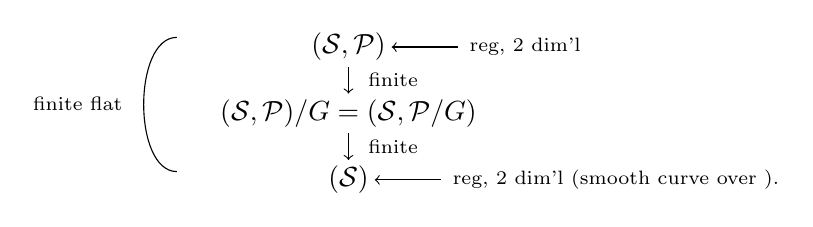
\begin{tikzpicture}[x=1em, y=1em, every node/.style={inner sep=2pt}]
\node (a) at (0,0) {$\Mfrak(\mathcal{S},\mathcal{P})$};
\node (b) at (0,-2.4) {$\Mfrak(\mathcal{S},\mathcal{P})/G = \Mfrak(\mathcal{S},\mathcal{P}/G)$};
\node (c) at (0,-4.8) {$\Mfrak(\mathcal{S})$};
\draw[->] (a) -- node[right=5pt] {\scriptsize finite} (b);
\draw[->] (b) -- node[right=5pt] {\scriptsize finite} (c);
\draw[<-] (a.east) -- ++(2.4,0) node[right=2pt] {\scriptsize reg, 2 dim'l};
\draw[<-] (c.east) -- ++(2.4,0) node[right=2pt] {\scriptsize reg, 2 dim'l (smooth curve over $\Z$).};
\draw[line width=0.4pt] (-6.2,0.35) .. controls (-7.8,0.35) and (-7.8,-4.5) .. (-6.2,-4.5);
\node[anchor=east] at (-7.95,-2.05) {\scriptsize finite flat};
\end{tikzpicture}
\end{center}
It suffices to show that $\Mfrak(\mathcal{S}, \mathcal{P})/G$ is regular two-dimensional, for then being finite over $\Mfrak(\mathcal{S})$ it will automatically be finite flat over $\Mfrak(\mathcal{S})$---once again, a finite map between regular schemes of the same dimension is necessarily flat. Because $\Mfrak(\mathcal{S}, \mathcal{P})$ is itself regular two-dimensional, it suffices to show that the finite morphism
\[
\begin{tikzcd}[column sep=large, row sep=large]
\Mfrak(\mathcal{S},\mathcal{P}) \arrow[d] \\
\Mfrak(\mathcal{S},\mathcal{P})/G = \Mfrak(\mathcal{S},\mathcal{P}/G)
\end{tikzcd}
\]
is finite and flat (by \cite[VII, 4.8]{AK1}).

Consider the set $\mathcal{U} \subset \Mfrak(\mathcal{S})$ of points $x$ such that for any $y \in \Mfrak(\mathcal{S}, \mathcal{P}/G)$ with $y \to x$, and any $z \in \Mfrak(\mathcal{S}, \mathcal{P})$ with $z \to y$, $\Mfrak(\mathcal{S}, \mathcal{P})$ is flat over $\Mfrak(\mathcal{S}, \mathcal{P}/G)$ at $z$. This set $\mathcal{U}$ is \emph{open} in $\Mfrak(\mathcal{S})$, because its complement is the image by the finite map $\Mfrak(\mathcal{S}, \mathcal{P}) \to \Mfrak(\mathcal{S})$ of the set of points in $\Mfrak(\mathcal{S}, \mathcal{P})$ where $\Mfrak(\mathcal{S}, \mathcal{P}) \to \Mfrak(\mathcal{S}, \mathcal{P}/G)$ is not flat, and this is a closed set (\cite[V, 5.5]{AK1}). We know that $\mathcal{U}$ contains all of $\Mfrak(\mathcal{S}) \tens{\Z} \Z[1/p]$. So it suffices to show that $\mathcal{U}$ contains all closed points of $\Mfrak(\mathcal{S})$ in characteristic $p$.

Let $x$ be a closed point of $\Mfrak(\mathcal{S})$ in characteristic $p$, corresponding to an elliptic curve $E_0$ over a finite field $k_0$, together with a level $\mathcal{S}$-structure.

Let us denote by $\cO$ the completion of the strict henselization of the local ring of $\Mfrak(\mathcal{S})$ at $x$, with respect to some choice $k_0 \hookrightarrow k$ of algebraic closure of $k_0$.

Let $E/k$ be $E_0 \tens{k_0} k$, and denote by $E/W(k)[[T]]$ the universal formal deformation of $E/k$. Then $\cO \simeq W(k)[[T]]$, with $E/W(k)[[T]]$ induced from the universal curve over $\Mfrak(\mathcal{S})$ by the base change $\Spec(\cO) \to \Mfrak(\mathcal{S})$.

We must show that after the base-change $\Spec(\cO) \to \Mfrak(\mathcal{S})$, we have a finite flat map:
\begin{center}
\footnotesize
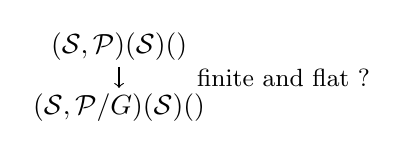
\begin{tikzpicture}[x=1em, y=1em, every node/.style={inner sep=2pt}]
\node (t) at (0,0) {$\Mfrak(\mathcal{S},\mathcal{P}) \tens{\Mfrak(\mathcal{S})} \Spec(\cO)$};
\node (u) at (0,-2.2) {$\Mfrak(\mathcal{S},\mathcal{P}/G) \tens{\Mfrak(\mathcal{S})} \Spec(\cO)$};
\draw[->] (t) -- (u);
\node[anchor=west] at (2.6,-1.1) {\small finite and flat ?};
\end{tikzpicture}
\end{center}
The source is by definition the scheme $\mathcal{P}_{E/W[[T]]}$, and the target is (using the flatness of $\Spec(\cO) \to \Mfrak(\mathcal{S})$)
\begin{align*}
\Mfrak(\mathcal{S}, \mathcal{P}/G) \tens{\Mfrak(\mathcal{S})} \Spec(\cO) &= \bigl(\Mfrak(\mathcal{S}, \mathcal{P})/G\bigr) \tens{\Mfrak(\mathcal{S})} \Spec(\cO) \\
&= \bigl(\Mfrak(\mathcal{S}, \mathcal{P}) \tens{\Mfrak(\mathcal{S})} \Spec(\cO)\bigr)/G \\
&= \bigl(\mathcal{P}_{E/W[[T]]}\bigr)/G .
\end{align*}
Thus we must show that
\[
\begin{tikzcd}[column sep=large, row sep=large]
\mathcal{P}_{E/W[[T]]} \arrow[d] \\
\bigl(\mathcal{P}_{E/W[[T]]}\bigr)/G
\end{tikzcd}
\]
is finite flat.

Because $\mathcal{P}$ satisfies Reg.~3, and the action of $G$ on $\mathcal{P}$ satisfies G-2, it follows by Serre-Tate theory that this morphism of $W[[T]]$-schemes is, up to isomorphism, of only two possible types, depending on whether $E/k$ is ordinary or supersingular. In particular, the question of whether it is finite flat depends only on whether $E/k$ is ordinary or not.

Because $\mathcal{U}$ is open, and contains $\Mfrak(\mathcal{S}) \tens{\Z} \Z[1/p]$, it suffices to show $\mathcal{U}$ contains all supersingular points in characteristic $p$. (Then it contains all nearby points, so some ordinary points, then all ordinary points.)

We now study the case of a supersingular $E/k$. In the notations of G-3, we must show that $A$ is a free module over $A^G$. For this, we argue as follows.

The map $G \to \Aut(A)$ is injective, because $A$ is flat over $\Z$ (being finite flat over $W[[T]]$) and, by G-1, $G$ acts freely on $\Spec(A \tens{\Z} \Z[1/p])$. Let $K$ denote the fraction field of $A$. Then $K^G$ is the fraction field of $A^G$ (replace denominators by their norms). By galois theory, $K$ is a $\#G$-dimensional vector space over $K^G$. Therefore if $A$ is spanned over $A^G$ by $\#G$ elements, these elements must be linearly independent over $K^G$, whence $A$ is a free module over $A^G$ of rank $\#G$.
\end{proof}

In order to apply (\ref{thm:7.5.1}), we will need the following result (with $n=2$).

\begin{kprop}\label{prop:7.5.2}
Let $A$ be a complete noetherian local ring which is regular of dimension $n$ and whose residue field is perfect. Let $G$ be a finite subgroup of $\Aut(A)$, such that every $g \in G$ acts trivially on the residue field of $A$. Suppose that $A$ admits a regular system of parameters $(x_1,\cdots,x_{n-1},y)$ such that for each $g \in G$ we have
\[
g(x_i) = x_i \quad \text{for} \quad i = 1,\cdots,n-1
\]
\[
g(y) \equiv y \times (\text{unit}) \mod (x_1,\cdots,x_{n-1}) .
\]
Then
\begin{enumerate}[(1)]
\item $A$ is free over $A^G$, with basis $1, y, y^2, \cdots, (y)^{\#G-1}$.
\item $A^G$ is a regular local ring of dimension $n$.
\item A set of parameters for $A^G$ is $(x_1,\cdots,x_{n-1},N(y))$ where $N(y)$ is the norm $\prod\limits_{g} g(y)$.
\end{enumerate}
\end{kprop}

\begin{proof}
Clearly the element $N(y)$ satisfies the congruence
\[
N(y) \equiv (y^{\#G})(\text{unit of } A) \mod (x_1,\cdots,x_{n-1}) ,
\]
and clearly the elements $(x_1,\cdots,x_{n-1},N(y))$ all lie in $A^G$.

We first claim that $A$ is spanned over $A^G$ by the $\#G$ elements
\[
1, y, \cdots, y^{\#G-1} .
\]
To prove this, it suffices by Nakayama to show that $A/\max(A^G) \cdot A$ is spanned over $A^G$ by these elements. We have an obvious inclusion
\[
\max(A^G) \supset (x_1,\cdots,x_{n-1},N(y)) ,
\]
and by our congruence on $N(y)$ we have
\[
\bigl(x_1,\cdots,x_{n-1},N(y)\bigr)A = \bigl(x_1,\cdots,x_{n-1},y^{\#G}\bigr) \cdot A .
\]
Therefore it suffices to show that
\[
A/(x_1,\cdots,x_{n-1},y^{\#G})A
\]
is spanned over $A^G$ by the lower powers of $y$. Because $A$ and $A^G$ have the same residue field $k$, the Cohen ring $C(k)$ maps to $A$ through $A^G$. Therefore it suffices if
\[
A/(x_1,\cdots,x_{n-1},y^{\#G})A
\]
is spanned over $C(k)$ by the lower powers of $y$, and this is visibly the case, just because $\max(A) = (x_1,\cdots,x_{n-1},y)$.

By considering the extension of fraction fields, we conclude that $A$ is free over $A^G$ on these elements, thus proving (1) and its consequence (2) (again by \cite[VII, 4.8]{AK1}). Now let $I \subset \max(A^G)$ be any ideal of $A^G$. Then $A/IA$ is free of rank $\#G$ over $A^G/I$. Therefore $I = \max(A^G)$ if and only if $A/IA$ has length $\leq \#G$. Applying this criterion to $I = (x_1,\cdots,x_{n-1},N(y))$, we get (3).
\end{proof}

\begin{kvar}\label{var:7.5.3}
Let $A$ be a complete noetherian regular local ring of dimension $n$ with perfect residue field, $G$ a finite subgroup of $\Aut(A)$ of the form $G_1 \times \cdots \times G_n$. Suppose that every $g \in G$ acts trivially on the residue field of $A$, and that there exists a regular system of parameters $(x_1,\cdots,x_n)$ for $A$ such that for each $i$, any element $g_i \in G_i$ satisfies
\[
\left\{
\begin{aligned}
g_i(x_j) &= x_j & & \text{if } j \neq i \\
g_i(x_i) &= x_i \times (\text{unit}) . & &
\end{aligned}
\right.
\]
Then $A^G$ is regular of dimension $n$, a set of parameters of $A^G$ is $(N_{G_1}(x_1),\cdots,N_{G_n}(x_n))$, and $A$ is free over $A^G$ on the $\#G$ monomials $\prod x_i^{w_i}$ with $0 \leq w_i \leq \#G_i - 1$.
\end{kvar}

\begin{proof}
Straightforward adaptation of the proof of the preceding proposition.
\end{proof}

% ------------------------------------------------------------------------------
% Section 7.6
% ------------------------------------------------------------------------------
\section{Applications to regularity}
\label{sec:7.6}

We now list some cases to which the Axiomatic Regularity of Quotients Theorem \ref{thm:7.5.1} applies via this proposition.

\begin{kthm}\label{thm:7.6.1}
\begin{enumerate}[(1)]
\item For any prime power $p^n$ with $n \geq 1$, and any subgroup $G$ of the ``semi-Borel''
\[
G \subset \left(\begin{smallmatrix} 1 & * \\ 0 & * \end{smallmatrix}\right) \subset \GL(2,\Z/p^n\Z)
\]
or any product subgroup $G = \left(\begin{smallmatrix} G_1 & 0 \\ 0 & G_2 \end{smallmatrix}\right)$ of the Cartan $\left(\begin{smallmatrix} * & 0 \\ 0 & * \end{smallmatrix}\right) \subset \GL(2,\Z/p^n\Z)$
the quotient $[\Gamma(p^n)]/G$ is regular two-dimensional, finite and flat over \Ell\ and under $[\Gamma(p^n)]$.
\item For any prime power $p^n$ with $n \geq 1$, and any two subgroups $G, H \subset (\Z/p^n\Z)^\times$, the quotients
\[
[\mathrm{bal.}\ \Gamma_1(p^n)]/(G \times H)
\]
\[
[\Gamma_1(p^n)]/G
\]
are regular two-dimensional, finite and flat over \Ell\ and under $[\mathrm{bal.}\ \Gamma_1(p^n)]$ (resp.\ $[\Gamma_1(p^n)]$).
\end{enumerate}
\end{kthm}

\begin{proof}
Simply apply the proposition (\ref{thm:7.5.1}) to $G$, and its variation (\ref{var:7.5.3}) to $G_1 \times G_2$ and to $G \times H$.
\end{proof}

% ------------------------------------------------------------------------------
% Section 7.7
% ------------------------------------------------------------------------------
\section{Summary of parameters at supersingular points (notations as in (\ref{sec:5.4}))}
\label{sec:7.7}

\begin{center}
{\scriptsize\setlength{\tabcolsep}{2pt}%
\begin{tabular}{@{}c|c|c@{}}
\hline
moduli problem & basic data & Parameters for $A$ \\
\hline
$[\Gamma(p^n)]$ & $(P, Q)$ & $X(P), X(Q)$ \\
\hline
$\begin{array}{@{}c@{}} {[\Gamma(p^n)]/G} \\[2pt] \text{with } G \subset \left(\begin{smallmatrix} 1 & * \\ 0 & * \end{smallmatrix}\right) \end{array}$ & $?$ & $X(P), N_G(X(Q))$ \\
\hline
$[\Gamma(p^n)]\big/\left(\begin{smallmatrix} G_1 & 0 \\ 0 & G_2 \end{smallmatrix}\right)$ & $?$ & $N_{G_1}(X(P)), N_{G_2}(X(Q))$ \\
\hline
$[\mathrm{bal.}\ \Gamma_1(p^n)]$ & $P \in E \rightleftarrows E' \ni P'$ & $X(P), X'(P')$ \\
\hline
$[\mathrm{bal.}\ \Gamma_1(p^n)]/G \times H$ & $?$ & $N_G(X(P)), N_H(X'(P'))$ \\
\hline
$\begin{array}{@{}c@{}} {[\Gamma_0(p^n)]} \text{ viewed as} \\[2pt] {[\mathrm{bal.}\ \Gamma_1(p^n)]/(\Z/p^n\Z)^\times} \\[2pt] {\times (\Z/p^n\Z)^\times} \end{array}$ & $E \underset{\pi^t}{\overset{\pi}{\rightleftarrows}} E'$ & $N_G(X(P)), N_H(X'(P'))$ \\
\hline
$\begin{array}{@{}c@{}} {[\Gamma_1(p^n)]} \text{ viewed as} \\[2pt] {[\mathrm{bal.}\ \Gamma_1(p^n)]/1 \times (\Z/p^n\Z)^\times} \end{array}$ & $P \in E \underset{\pi^t}{\overset{\pi}{\rightleftarrows}} E'\,(\text{forget } P')$ & $X(P), N(X'(P'))$ \\
\hline
$[\Gamma_1(p^n)]$ & $P \in E$ & $T, X(P)$ \\
\hline
$\begin{array}{@{}c@{}} {[\Gamma_0(p^n)]} \text{ viewed as} \\[2pt] {[\Gamma_1(p^n)]/(\Z/p^n\Z)^\times} \end{array}$ & $(\text{forget } P)\ E \underset{\pi^t}{\overset{\pi}{\rightleftarrows}} E'$ & $T, N(X(P))$ \\
\hline
\end{tabular}}
\end{center}

\begin{krem}\label{rem:7.7.1}
Depending upon how we view $\Gamma_0(p^n)$ and $\Gamma_1(p^n)$, we get different sets of parameters at the supersingular points, depending on whether we think of the objects being classified as extra data on a single $E$, or as extra data on a diagram $E \rightleftarrows E'$. We give below still another set of parameters for $\Gamma_0(p^n)$ at the supersingular points, namely the ``$T$-invariants'' of the source and target.
\end{krem}

% ------------------------------------------------------------------------------
% Section 7.8
% ------------------------------------------------------------------------------
\section{More parameters for $[\Gamma_0(p^n)]$, $n \geq 1$, at supersingular points}
\label{sec:7.8}

\kmitem\label{item:7.8.1}
Fix a supersingular elliptic curve $E_0/k$, $k$ a perfect field of characteristic $p$, $E/W[[T]]$ its universal formal deformation, and $E_1/W[[T_1]]$ the universal formal deformation of $E_1 = E_0^{(p^n)}$. We know that $[\Gamma_0(p^n)]_{E/W[[T]]}$ is a closed subscheme of $[p^n\text{-Isog}]_{E/W[[T]]}$, and that this latter is a closed subscheme of $\Spec(W[[T,T_1]])$, by the constructions
\[
(\text{cyclic } p^n\text{-isogeny}) \mapsto (\text{source}, \text{target}) .
\]
We denote by $A$ the complete two-dimensional regular local ring such that
\[
\Spec(A) = [\Gamma_0(p^n)]_{E/W[[T]]} .
\]
Then $A$ is a quotient of $W[[T,T_1]]$, and we have already seen (\ref{sec:7.7}) that $A$ admits a regular sequence of parameters of the form $(T,Y)$ for some $Y$ (e.g., $Y = N(X(P))$, viewing $[\Gamma_0(p^n)]$ as $[\Gamma_1(p^n)]/(\Z/p^n\Z)^\times$).

\begin{kprop}\label{prop:7.8.2}
The elements $(T,T_1)$ are a regular sequence of parameters for $A$.
\end{kprop}

\begin{proof}
This is true for any quotient of $W[[T,T_1]]$ which is regular of dimension two, which is finite and flat over $W[[T]]$ of degree $\geq 2$, and admits $(T,Y)$ as parameters for some $Y$. For $A$ is necessarily of the form $W[[T,T_1]]/(f)$ where $f$ is part of a regular system of parameters of $W[[T,T_1]]$. So modulo $m^2$, $f$ is a $k$-linear combination of $p,T,T_1$. Our assertion is that the coefficient of $p$ is non-zero (then $(f,T,T_1)$ is a system of parameters for $W[[T,T_1]]$). If not, then
\[
f = aT + bT_1 \mod m^2 .
\]
If $b \neq 0$, then $(f,T,p)$ is a system of parameters for $W[[T,T_1]]$, whence $(T,p)$ would be a system of parameters for $A$. This is impossible if $A$ is to be finite flat over $W[[T]]$ of degree $\geq 2$. If $b = 0$, then $a \neq 0$ (otherwise $A$ won't be regular), so we can take $a = 1$, and then $\bmod f$ we find $T \in (\max(A))^2$, contradicting the fact that $T$ is part of a regular system of parameters for $A$.
\end{proof}

% ------------------------------------------------------------------------------
% Section 7.9
% ------------------------------------------------------------------------------
\section{Detailed study of the congruence quotients $[\Gamma_0(p^n); a, b]$ of $[\mathrm{bal.}\ \Gamma_1(p^n)]$}
\label{sec:7.9}

\kmitem\label{item:7.9.1}
In this section, we will give the modular interpretation of the quotient of $[\mathrm{bal.}\ \Gamma_1(p^n)]$ by any subgroup of $(\Z/p^n\Z)^\times \times (\Z/p^n\Z)^\times$ of the form $\Gamma \times \Gamma'$, where $\Gamma$ and $\Gamma'$ are both standard congruence subgroups of $(\Z/p^n\Z)^\times$.

Recall (\ref{km:6.7.6}, \ref{thm:6.7.9}) that if
\begin{equation}\label{eq:7.9.1.1}
E_0 \kmdual{\pi}{\lambda = \pi^t} E_n
\end{equation}
is a dual pair of cyclic $p^n$-isogenies between elliptic curves over any base $S$, then both $\pi$ and $\lambda$ admit ``standard'' factorization into (necessarily) cyclic $p$-isogenies, and these standard factorizations are dual to each other: we have a diagram
\begin{equation}\label{eq:7.9.1.2}
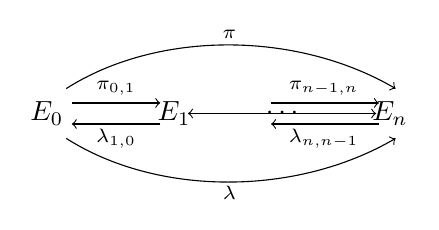
\begin{tikzpicture}[x=1em, y=1em, every node/.style={inner sep=1pt}]
\node (E0) at (0,0) {$E_0$};
\node (E1) at (4.6,0) {$E_1$};
\node (En) at (12.4,0) {$E_n$};
\node (Ed) at (8.5,0) {$\cdots$};
\draw[->] (0.9,0.38) -- (4.1,0.38);
\node at (2.5,0.92) {\scriptsize $\pi_{0,1}$};
\draw[->] (4.1,-0.38) -- (0.9,-0.38);
\node at (2.5,-0.92) {\scriptsize $\lambda_{1,0}$};
\draw[<->] (5.1,0) -- (11.9,0);
\draw[->] (8.1,0.38) -- (12.0,0.38);
\node at (10.0,0.92) {\scriptsize $\pi_{n-1,n}$};
\draw[->] (12.0,-0.38) -- (8.1,-0.38);
\node at (10.0,-0.92) {\scriptsize $\lambda_{n,n-1}$};
\draw[->] (0.7,0.9) .. controls (4.0,3.0) and (9.0,3.0) .. (12.6,0.9);
\node at (6.6,2.85) {\scriptsize $\pi$};
\draw[->] (0.7,-0.9) .. controls (4.0,-3.0) and (9.0,-3.0) .. (12.6,-0.9);
\node at (6.6,-2.85) {\scriptsize $\lambda$};
\end{tikzpicture}
\end{equation}
\addtocounter{equation}{1}% the book's (7.9.1.3) is not printed
where $(\pi_{0,1},\cdots,\pi_{n-1,n})$ is the standard factorization of $\pi$, $(\lambda_{n,n-1},\cdots,\lambda_{1,0})$ is the standard factorization of $\lambda$, and where for $1 \leq a \leq n$, we have
\begin{equation}\label{eq:7.9.1.4}
\lambda_{a,a-1} = (\pi_{a-1,a})^t .
\end{equation}
For brevity, we denote, for $0 \leq i < j \leq n$, the partial composites
\begin{equation}\label{eq:7.9.1.5}
E_i \kmdual{\pi_{i,j}}{\lambda_{j,i}} E_j
\end{equation}
i.e.,
\[
\pi_{i,j} = \pi_{j-1,j} \circ \pi_{j-2,j-1} \circ \cdots \pi_{i,i+1}
\]
\[
\lambda_{j,i} = \lambda_{i+1,i} \circ \lambda_{i+2,i+1} \cdots \circ \lambda_{j,j-1} .
\]

\begin{kprop}\label{prop:7.9.2}
Let $P \in (\Ker \pi)(S)$ be a generator of $\Ker \pi$, and let $Q \in (\Ker \lambda)(S)$ be a generator of $\Ker(\lambda)$. Then
\begin{enumerate}[(1)]
\item for every $(a,b)$ with $0 \leq a, b \leq n-1$ and $0 \leq a+b \leq n-1$, $p^b \pi_{0,a}(P)$ generates $\Ker(\pi_{a,n-b})$, and $p^a \lambda_{n,n-b}(Q)$ generates $\Ker(\lambda_{n-b,a})$.
\item The canonical pairings $\langle\ ,\ \rangle$ of these points are related by
\[
\langle p^b \pi_{0,a}(P), p^a \lambda_{n,n-b}(Q) \rangle_{\pi_{a,n-b}} = (\langle P, Q \rangle_\pi)^{p^{a+b}} ,
\]
and $\langle P, Q \rangle_\pi$ is a ``primitive'' $p^n$'th root of unity.
\end{enumerate}
\end{kprop}

\begin{proof}
Assertion (1) is a special case of the Backing-Up Theorem (\ref{thm:6.7.11}).

Assertion (2) is physically obvious if $p$ is invertible, and as $[\mathrm{bal.}\ \Gamma_1(p^n)]$ is flat over $\Z$ it follows in general.
\end{proof}

\begin{kprop}\label{prop:7.9.3}
Let $0 \leq a, b \leq n$ be two integers. Let $P_a \in \Ker(\pi_{a,n})(S)$ be a generator of $\Ker(\pi_{a,n})$, and let $Q_{n-b} \in \Ker(\lambda_{n-b,0})$ be a generator of $\Ker(\lambda_{n-b,0})$.
\begin{center}
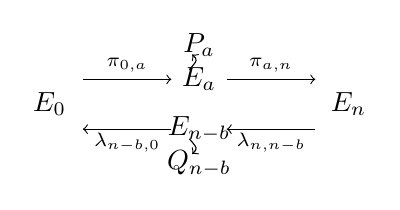
\begin{tikzpicture}[x=1em, y=1em, every node/.style={inner sep=2pt}]
\node (E0) at (0,0) {$E_0$};
\node (Ea) at (5.4,0.9) {$E_a$};
\node (Enb) at (5.4,-0.9) {$E_{n-b}$};
\node (En) at (10.8,0) {$E_n$};
\node (Pa) at (5.4,2.15) {$P_a$};
\node (Qnb) at (5.4,-2.15) {$Q_{n-b}$};
\draw[->] (1.2,0.9) -- (4.4,0.9);
\node at (2.8,1.4) {\scriptsize $\pi_{0,a}$};
\draw[->] (4.4,-0.9) -- (1.2,-0.9);
\node at (2.8,-1.4) {\scriptsize $\lambda_{n-b,0}$};
\draw[->] (6.4,0.9) -- (9.6,0.9);
\node at (8.0,1.4) {\scriptsize $\pi_{a,n}$};
\draw[->] (9.6,-0.9) -- (6.4,-0.9);
\node at (8.0,-1.4) {\scriptsize $\lambda_{n,n-b}$};
\draw[->] (5.05,1.25) .. controls (5.35,1.6) .. (5.15,1.8);
\draw[->] (5.05,-1.25) .. controls (5.35,-1.6) .. (5.15,-1.8);
\end{tikzpicture}
\end{center}
Then
\begin{enumerate}[(1)]
\item for $0 \leq c \leq a$, $\lambda_{a,c}(P_a)$ generates $\Ker(\pi_{c,n+c-a})$.
\item for $0 \leq d \leq b$, $\pi_{n-b,n-b+d}(Q_{n-b})$ generates $\Ker(\lambda_{n-b+d,d})$.
\item If $a \leq b$, then for $0 \leq c \leq a$ the canonical pairing
\[
\langle p^{b-a} \lambda_{a,c}(P_a),\ \pi_{n-b,n-b+c}(Q_{n-b}) \rangle
\]
is a ``primitive'' $p^{n-b}$'th root of unity, independent of the choice of $c$.
\item[(3 bis)] If $a \geq b$, then for $0 \leq d \leq b$ the canonical pairing
\[
\langle \lambda_{a,a-d}(P_a),\ p^{a-b} \pi_{n-b,n-d}(Q_{n-b}) \rangle
\]
is a ``primitive'' $p^{n-a}$'th root of unity, independent of the choice of $d$.
\end{enumerate}
\end{kprop}

\begin{proof}
The assertion is f.p.p.f. local on $S$. So we may assume we are given a point $P_0 \in (\Ker \pi)(S)$ such that $\pi_{0,a}(P_0) = P_a$, and a point $Q_n \in (\Ker \lambda)(S)$ such that $\lambda_{n,n-b}(Q_n) = Q_{n-b}$. By the Backing-Up Theorem (\ref{thm:6.7.11}), $P_0$ generates $\Ker \pi$, and $Q_n$ generates $\Ker \lambda$. The result now follows from the previous proposition applied to $P_0, Q_n$.
\end{proof}

\begin{definition}\label{def:7.9.4}
For integers $0 \leq a, b \leq n$, we define a $[\Gamma_0(p^n); a, b]$ structure on an elliptic curve $E/S$ to be a cyclic $p^n$-isogeny $\pi : E_0 \to E_n$ with dual $\lambda = \pi^t$ together with points $P_{n-a} \in (\Ker \pi_{n-a,n})(S)$ and $Q_b \in (\Ker \lambda_{b,0})(S)$ which generate these kernels
\[
E_0 \kmdual{\pi_{0,n-a}}{\lambda_{b,0}} E_{n-a} \kmdual{\pi_{n-a,n}}{\lambda_{n,b}} E_n .
\]
\end{definition}

We denote by
\begin{equation}\label{eq:7.9.4.1}
[\Gamma_0(p^n); a, b]
\end{equation}
the corresponding moduli problem. It is naturally a moduli problem over $\Z[\zeta_{p^{\min(a,b)}}]$, by the $\langle\ ,\ \rangle$ pairing (cf.\ (3), (3 bis) of \ref{prop:7.9.3}).

There are natural morphisms of moduli problems
\begin{equation}\label{eq:7.9.4.2}
\begin{tikzcd}[row sep=large]
{[\mathrm{bal.}\ \Gamma_1(p^n)] = [\Gamma_0(p^n); n, n]} \arrow[d] \\
{[\Gamma_0(p^n); a, b]} \arrow[d] \\
{[\Gamma_0(p^n)]}
\end{tikzcd}
\end{equation}
defined by
\begin{equation}\label{eq:7.9.4.3}
\begin{tikzcd}[row sep=large, every label/.append style={font=\scriptsize}]
{(E_0 \kmdual{\pi}{\lambda} E_n;\ P_0, Q_n)} \arrow[d] \\
{(E_0 \kmdual{\pi}{\lambda} E_n;\ P_{n-a} = \pi_{0,n-a}P_0;\ Q_b = \lambda_{n,b}Q_n)} \arrow[d] \\
{(E_0 \kmdual{\pi}{\lambda} E_n) .}
\end{tikzcd}
\end{equation}
Let us temporarily denote by
\begin{equation}\label{eq:7.9.4.4}
\Gamma(a) \subset (\Z/p^n\Z)^\times
\end{equation}
the subgroup of elements $\equiv 1 \bmod p^a$, so that we have a tautological exact sequence
\[
1 \to \Gamma(a) \to (\Z/p^n\Z)^\times \to (\Z/p^a\Z)^\times \to 1 .
\]

\begin{klem}\label{lem:7.9.5}
The map
\[
[\mathrm{bal.}\ \Gamma_1(p^n)] \to [\Gamma_0(p^n); a, b]
\]
is equivariant for the natural action of $\Gamma(a) \times \Gamma(b)$ on $[\mathrm{bal.}\ \Gamma_1(p^n)]$, and its trivial action on $[\Gamma_0(p^n); a, b]$.
\end{klem}

\begin{proof}
We must show that if $\alpha \equiv 1 \bmod p^a$, then $\pi_{0,n-a}(P_0) = \pi_{0,n-a}(\alpha P_0)$ (and similarly for $b$ and $Q_0$). Writing $\alpha = 1 + p^a\gamma$, this amounts to
\[
\pi_{0,n-a}(p^a P_0) = 0 .
\]
But $p^a P_0$ is in fact a generator of $\Ker(\pi_{0,n-a})$.
\end{proof}

There is also an obvious action of the group $(\Z/p^a\Z)^\times \times (\Z/p^b\Z)^\times$ on $[\Gamma_0(p^n); a, b]$, defined by having $(\alpha,\beta)$ move $(E_0 \rightleftarrows E_n; P_{n-a}, Q_b)$ to $(E_0 \rightleftarrows E_n; \alpha P_{n-a}, \beta Q_b)$.

\begin{kthm}\label{thm:7.9.6}
For any $0 \leq a, b \leq n$, the moduli problem $[\Gamma_0(p^n); a, b]$ is regular two-dimensional, finite and flat over $[\Gamma_0(p^n)]$, finite and flat under $[\mathrm{bal.}\ \Gamma_1(p^n)]$. The natural maps
\begin{center}
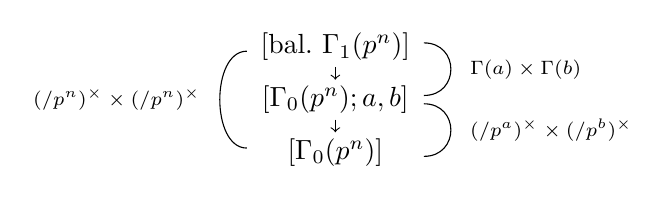
\begin{tikzpicture}[x=1em, y=1em, every node/.style={inner sep=2pt}]
\node (A) at (0,0) {$[\mathrm{bal.}\ \Gamma_1(p^n)]$};
\node (B) at (0,-1.9) {$[\Gamma_0(p^n); a, b]$};
\node (C) at (0,-3.8) {$[\Gamma_0(p^n)]$};
\draw[->] (A) -- (B);
\draw[->] (B) -- (C);
\draw[line width=0.4pt] (-3.2,-0.15) .. controls (-4.5,-0.15) and (-4.5,-3.65) .. (-3.2,-3.65);
\node[anchor=east] at (-4.65,-1.9) {\scriptsize $(\Z/p^n\Z)^\times \times (\Z/p^n\Z)^\times$};
\draw[line width=0.4pt] (3.2,0.15) .. controls (4.5,0.15) and (4.5,-1.75) .. (3.2,-1.75);
\node[anchor=west] at (4.65,-0.8) {\scriptsize $\Gamma(a) \times \Gamma(b)$};
\draw[line width=0.4pt] (3.2,-2.05) .. controls (4.5,-2.05) and (4.5,-3.95) .. (3.2,-3.95);
\node[anchor=west] at (4.65,-3.0) {\scriptsize $(\Z/p^a\Z)^\times \times (\Z/p^b\Z)^\times$};
\end{tikzpicture}
\end{center}
define isomorphisms
\[
[\mathrm{bal.}\ \Gamma_1(p^n)]/\Gamma(a) \times \Gamma(b) \xrightarrow{\ \sim\ } [\Gamma_0(p^n); a, b]
\]
\[
[\Gamma_0(p^n); a, b]/(\Z/p^a\Z)^\times \times (\Z/p^b\Z)^\times \xrightarrow{\ \sim\ } [\Gamma_0(p^n)] .
\]
\end{kthm}

\begin{proof}
It suffices to establish that $[\Gamma_0(p^n); a, b]$ is regular two-dimensional and finite over \Ell. Then the finite flatness is automatic. The statements about quotients result from the physically obvious fact that they are true outside of $p$ (compare the proof of (\ref{thm:7.4.2})). We prove the regularity by a straightforward application of the Axiomatic Regularity Theorem (\ref{thm:5.2.1}). Axioms Reg.~1, Reg.~2, Reg.~3, and Reg.~4A are easily checked. Suppose both $a, b \geq 1$. Then we verify Reg.~4B bis by observing that the (formal-group coordinates of the) points $P_{n-a}, Q_b$ provide parameters. For consider, over an artin local ring $R$ with perfect residue field $k$ of characteristic $p$, a cyclic $p^n$-isogeny
\[
E_0 \kmdual{\pi_{0,1}}{\lambda_{1,0}} E_1 \kmdual{\cdots}{\cdots} \cdots \kmdual{\pi_{n-1,n}}{\lambda_{n,n-1}} E_n
\]
such that $0$ generates $\Ker(\pi_{n-a,n})$, and such that $0$ generates $\Ker(\lambda_{b,0})$. By the Backing-up Theorem (\ref{thm:6.7.11}), $0$ generates $\Ker(\pi)$, and it generates $\Ker(\lambda)$. Therefore $R$ is a $k$-algebra, and both $\Ker(\pi) = \Ker(F^n)$, $\Ker(\lambda) = \Ker(F^n)$; whence
\[
E_0 \simeq (E_n)^{(p^n)} \quad \text{via} \quad \lambda
\]
\[
E_n \simeq (E_0)^{(p^n)} \quad \text{via} \quad \pi
\]
so that $E_0 \simeq E_0^{(p^{2n})}$, whence $E_0/R$ is constant, $E_n/R$ is constant, and the isogenies $\pi_{i,i+1}, \lambda_{i+1,i}$ are all $F$.

If $a = b = 0$, then $[\Gamma_0(p^n); 0, 0]$ is just $[\Gamma_0(p^n)]$, and the theorem is already proven. If one but not both of $(a,b)$ vanishes, say $a > 0$, $b = 0$, then ``$T_0$'' and ``$X(P_{n-a})$'' give parameters. For if $P_{n-a} = 0$, then $0$ generates $\Ker(\pi)$, whence $p = 0$, $R$ is a $k$-algebra and $\Ker(\lambda) = \Ker(F^n)$. Because ``$T_0$'' $= 0$, we also have $E_0$ constant over $R$.

If $a = 0$ and $b > 0$, then ``$T_n$'' and ``$X(Q_b)$'' give parameters, by the symmetric argument.
\end{proof}


% ------------------------------------------------------------------------------
% Appendix (A7)
% ------------------------------------------------------------------------------
\kmappendixA{A7}{Appendix: Base-change for rings of invariants}{APPENDIX: BASE CHANGE FOR RINGS OF INVARIANTS}
\label{sec:A.7}

\subsection{Sufficient conditions}

Let $R$ be a ring, $A$ an $R$-algebra, and $G$ a finite group which acts on $A$ by $R$-linear ring automorphisms. We denote by $A^G \subset A$ the $R$-subalgebra of all $G$-invariants. For any $R$-algebra $R'$, the group $G$ acts $R'$-linearly on $A \tens{R} R'$ [by $g(a \otimes r') = g(a) \otimes r'$], and we have a natural $R'$-homomorphism
\[
A^G \tens{R} R' \to (A \tens{R} R')^G .
\]
Let us denote by
\[
*(A,G,R,R')
\]
the statement that the above map is an isomorphism, and by
\[
*(A,G,R)
\]
the statement that the above map is an isomorphism for every $R$-algebra $R'$.

\begin{appthm}\label{thm:A7.1.1}
Let $R$ be a ring, $A$ an $R$-algebra, and $G$ a finite group operating on $A$ by $R$-algebra automorphisms. Suppose that $G$ acts freely on $A$ in the sense that for any non-zero $R$-algebra $R'$, and any element $g \neq id$ of $G$, $g$ operates without fixed points on the set $\Hom_{R\text{-alg}}(A,R')$. Then $A$ is a finite etale $G$-torsor over $A^G$, and the natural map
\[
A \tens{A^G} A \to \prod_{g \in G} A
\]
\[
x \otimes y \mapsto (\cdots, x \otimes g(y), \cdots)
\]
is an isomorphism of left $A$-algebras.
\end{appthm}

\begin{proof}
In the absence of noetherian hypotheses, this is rather delicate. See (\cite[III, Expos\'e V, Thm.~4.1]{SGA}), or \cite[III, \S2,6.1]{DeGa} for the proof.
\end{proof}

\begin{appcor}\label{cor:A7.1.2}
Hypotheses as in A7.1.1 above, $*(A,G,R)$ holds.
\end{appcor}

\begin{proof}
By the above theorem, $A$ is a finite etale $G$-torsor over $A^G$. For any $R$-algebra $R'$, if we make the extension of scalars $A^G \to A^G \tens{R} R'$, we obtain a finite etale $G$-torsor over $A^G \tens{R} R'$, namely $A \tens{R} R'$. But if $A \tens{R} R'$ is a finite etale $G$-torsor over $A^G \tens{R} R'$, then we certainly have
\[
(A \tens{R} R')^G = A^G \tens{R} R' ,
\]
i.e., $*(A,G,R,R')$ holds for any $R'$.
\end{proof}

\begin{appprop}\label{prop:A7.1.3}
\begin{enumerate}[label=(\arabic*), start=0]
\item For any $R$-algebra $R'$, $*(A,G,R) \Rightarrow *(A \tens{R} R', G, R')$.
\item If $R'$ is flat over $R$, then $*(A,G,R,R')$ holds.
\item If $R'$ is faithfully flat over $R$, then $*(A,G,R) \Longleftrightarrow *(A \tens{R} R', G, R')$.
\item If $\#G$ is invertible in $R'$, then $*(A,G,R,R')$ holds.
\item If $\#G$ is invertible in $R$, then $*(A,G,R)$ holds.
\end{enumerate}
\end{appprop}

\begin{proof}
Assertion (0) is essentially a tautology. For if $*(A,G,R)$ holds, then for any homomorphisms $R \to R' \to R''$, we have a commutative diagram
\begin{center}
\footnotesize
\begin{tikzcd}[column sep=small, row sep=large, every label/.append style={font=\scriptsize}]
{(A \tens{R} R')^G \tens{R'} R''} \arrow[r] \arrow[d, "\wr"'] & {\bigl((A \tens{R} R') \tens{R} R''\bigr)^G} \arrow[d, "\wr"] \\
{(A^G \tens{R} R') \tens{R'} R''} \arrow[r, "\sim"] & {A^G \tens{R} R''} \arrow[r, "\sim"] & {(A \tens{R} R'')^G}
\end{tikzcd}
\end{center}
Assertion (1) holds simply because $A^G$ is a kernel:
\[
0 \to A^G \to A \xrightarrow{\ \oplus(1-g)\ } \bigoplus_{g} A
\]
is an exact sequence of $R$-modules. For (2), let $R \to R''$ be an $R$-algebra. Then $R''' = R' \tens{R} R''$ is faithfully flat over $R''$. Consider the exact sequence of $R''$-modules
\[
0 \to \Ker \to A^G \tens{R} R'' \to (A \tens{R} R'')^G \to \Coker \to 0 .
\]
Because $R'''$ is flat over $R''$, we may infer using (1) an exact sequence
\[
0 \to \Ker \tens{R''} R''' \to A^G \tens{R} R''' \to (A \tens{R} R''')^G \to \Coker \tens{R''} R''' \to 0 .
\]
Because $R'''$ is faithfully flat over $R''$, the two end terms vanish after $\otimes R'''$ if and only if they vanished before.

To prove (3) and (4), we argue as follows. It suffices to prove (4), for if $\#G$ is invertible in $R'$, then $R \to R'$ factors as
\[
R \to R[1/\#G] \to R' .
\]
The first arrow is a localization, so flat, and (4) covers the second. To prove (4), simply use the divided trace
\[
T = \frac{1}{\#G}\sum_{g} g \qquad \in R[G]
\]
as a projection to exhibit $A^G$ as a direct factor of $A$ as $R$-module:
\[
A = A^G \oplus (1-T)(A) .
\]
Therefore the map
\[
A^G \tens{} R' \to (A \tens{} R')^G \subset A \tens{} R'
\]
is injective. It is also surjective, because given an element
\[
\sum a_i \tens{} r_i' \in (A \tens{} R')^G ,
\]
it is the image of the element
\[
\sum T(a_i) \tens{} r_i' \in A^G \tens{} R' .
\]
\end{proof}

\begin{appprop}\label{prop:A7.1.4}
Let $R$ be a discrete valuation ring, with uniformizing parameter $\pi$. Consider the conditions:
\begin{enumerate}[(1)]
\item $*(A,G,R)$ holds.
\item $*(A,G,R,R/\pi^n R)$ holds for all $n \geq 1$.
\item $*(A/\pi^n A, G, R/\pi^n R)$ holds for all $n \geq 1$.
\end{enumerate}
Then we always have the implications
\[
(1) \Longleftrightarrow (2) \Longrightarrow (3) .
\]
If the fraction field of $R$ has characteristic zero, and if $A$ is $R$-flat, then
\[
(1) \Longleftrightarrow (2) \Longleftrightarrow (3) .
\]
\end{appprop}

\begin{proof}
Trivially, (1) $\Rightarrow$ (2), and (1) $\Rightarrow$ (3) by part (0) of the preceding proposition. Let us prove (2) $\Rightarrow$ (1). To prove (1), it obviously suffices to prove that for any $R$-module $M$, the natural map of $R$-modules
\[
A^G \tens{R} M \to (A \tens{R} M)^G
\]
is an isomorphism. Expressing $M$ as the direct limit of its finitely generated submodules, and noting that both source and target commute with direct limits, we are reduced to checking when $M$ is a finitely generated $R$-module. Because $R$ is a discrete valuation ring, such an $M$ is a direct sum of $R$'s and of $R/\pi^n R$'s for various $n \geq 1$.

Let us now prove that (3) $\Rightarrow$ (2). Let us denote by $k$ the $\pi$-adic valuation of $\#G$:
\[
\#G = \pi^k \times (\text{unit in } R) .
\]
We will show that (3)$(n+k)$ $\Rightarrow$ (2)$(n)$. Consider the commutative diagram
\begin{center}
\begin{tikzcd}[column sep=large, row sep=large]
& {(A/\pi^{n+k}A)^G \tens{R} (R/\pi^n R)} \arrow[dl] \arrow[dr] & \\
A^G \arrow[rr, "\Theta"'] & & {(A/\pi^n A)^G}
\end{tikzcd}
\end{center}
We first show that $\Theta$ is surjective. Given an element
\[
a_n \in (A/\pi^n A)^G ,
\]
lift it to an element
\[
a_{n+k} \in (A/\pi^{n+k}A)^G , \qquad a_{n+k} \bmod \pi^n = a_n ,
\]
then choose
\[
a \in A , \qquad a \bmod \pi^{n+k} = a_{n+k} .
\]
Because $a_{n+k}$ is $G$-invariant, we have the congruence
\[
(\#G)(a) = \trace_G(a) \bmod \pi^{n+k}A .
\]
Because $A$ is $R$-flat, this shows that the divided trace of $a$ lies in $A$, and satisfies the congruence
\[
a \equiv T(a) \bmod \pi^n A .
\]
It remains to show that the kernel of $\Theta$ is $\pi^n(A^G)$. Because $(A/\pi^n A)^G$ is a subring of $A/\pi^n A$, the kernel of $\Theta$ is $A^G \cap \pi^n A$. Let $a \in \Ker$. Then $a = \pi^n b$, with $a \in A^G$ and $b \in A$. Then $\pi^n(g(b)-b) = 0$ for $g \in G$, whence $A$ being $R$-flat, $b \in A^G$.
\end{proof}

\subsection{Radicality}

\begin{appprop}[O. Gabber]\label{prop:A7.2.1}
In the situation of A7.1, let $p$ be a prime number, $p^n$ the highest power of $p$ which divides $\#G$. If $R'$ is a $\Z_{(p)}$-algebra ($\Z_{(p)} = $ the localization of $\Z$ at $(p) = \Q \cap \Z_p$), then the canonical homomorphism
\[
A^G \tens{R} R' \to (A \tens{R} R')^G
\]
satisfies
\begin{enumerate}[(1)]
\item every element of the target ring has $p^n$'th power in the image.
\item every element of the kernel has $p^n$'th power equal to zero.
\end{enumerate}
\end{appprop}

\begin{proof}
We first reduce to the case when $R$ is itself a $\Z_{(p)}$-algebra. For this, factor $R \to R'$ as
\[
R \to R \tens{\Z} \Z_{(p)} \to R' .
\]
Because the first map is flat, we may, by \ref{prop:A7.1.3} (1), replace $R$ by $R \tens{\Z} \Z_{(p)}$.

We next reduce to the case when $R' = R/I$ for some ideal $I$ of $R$. For this, write $R'$ as the quotient of a polynomial ring $R'' = R[X_1,X_2,\cdots]$ over $R$, possibly in infinitely many variables, by an ideal $I$. Then factor $R \to R'$ as
\[
R \to R'' \to R''/I .
\]
Again the first map is flat (indeed $R''$ is a free $R$-module), so we may, by \ref{prop:A7.1.3} (1), replace $R$ by $R''$.

Thus we may assume that $R$ is a $\Z_{(p)}$-algebra, and that $R' = R/I$. We first prove (1), that the image of
\[
A^G/IA^G \to (A/IA)^G
\]
contains all $p^n$'th powers. Let
\[
\tilde a \in (A/IA)^G ,
\]
and choose an element
\[
a \in A , \qquad a \equiv \tilde a \bmod IA .
\]
We will show that $a^{p^n}$ lies in $A^G$. For this, we argue as follows. Because $\tilde a$ is $G$-invariant, we have a congruence of polynomials
\[
\prod_{g \in G} (1 + g(a)X) \equiv (1 + aX)^{\#G} \bmod IA[X] .
\]
The left-hand polynomial visibly has coefficients in $A^G$. Equating coefficients of $X^{p^n}$, we obtain
\[
(\text{an element of } A^G) \equiv \binom{\#G}{p^n} a^{p^n} \bmod IA .
\]
By hypothesis, $\#G = p^n N$ with $(N,p) = 1$, whence
\[
\binom{\#G}{p^n} \equiv N \bmod p\Z ,
\]
so that
\[
\binom{\#G}{p^n} = \text{a unit in } \Z_{(p)} .
\]
We next show that every element in the kernel of
\[
A^G/IA^G \to (A/IA)^G
\]
has $p^n$'th power equal to zero. Thus let
\[
a \in A^G \cap (IA) ,
\]
say
\[
a = \sum f_i a_i \quad \text{with} \quad f_i \in I,\ a_i \in A .
\]
Because $a$ is $G$-invariant, we have an equality of polynomials
\[
\prod_{g \in G} (1 + g(a)X) = (1 + aX)^{\#G} .
\]
Writing $a = \sum f_i a_i$, and momentarily viewing the $f_i$ as indeterminates, we see that in the polynomial
\[
\prod_{g \in G} (1 + g(a)X) = \prod_{g \in G} \Bigl(1 + \bigl(\sum f_i g(a_i)\bigr)X\Bigr) ,
\]
the coefficient of $X^j$ is a sum, with $A^G$-coefficients, of monomials of degree $j$ in the $f_i$'s. In particular, for $j > 0$, the coefficient of $X^j$ lies in $IA^G$. Again equating coefficients of $X^{p^n}$, we find
\[
\binom{\#G}{p^n} a^{p^n} \in IA^G ,
\]
as required.
\end{proof}

\begin{appcor}\label{cor:A7.2.2}
For any $R \to R'$, the map
\[
A^G \tens{R} R' \to (A \tens{R} R')^G
\]
is bijective on geometric points.
\end{appcor}

\begin{proof}
We reduce immediately to the case where $R'$ is itself an algebraically closed field $K$. If $K$ has characteristic zero, the map $A^G \tens{R} K \to (A \tens{R} K)^G$ is an isomorphism (because $\#G$ is invertible in $K$), while if $K$ has characteristic $p > 0$, this map is surjective and radicial (by \ref{prop:A7.2.1}).
\end{proof}
